\documentclass[a1paper,fontscale=.47]{baposter}

%%%%lualatex on
%\usepackage{luatextra}
\usepackage{fontspec}
%Ligatures={Contextual, Common, Historical, Rare, Discretionary}
\setmainfont[Mapping=tex-text]{Lora}

%%%lua off
%\usepackage[utf8x]{inputenc}
%\usepackage[T1]{fontenc} 
%\usepackage{lmodern}

\usepackage{enumerate}
\usepackage[english]{babel}
\usepackage{graphicx} %to insert pictures
\usepackage{color} %to set colors
\usepackage{latexsym}
\usepackage{caption}
\usepackage{multicol}
\usepackage{amsmath}

\usepackage{float}
\usepackage{booktabs}

\newcommand{\specialcell}[2][c]{%
  \begin{tabular}[#1]{@{}c@{}}#2\end{tabular}}


\makeatletter
\let\oldabs\abs
\def\abs{\@ifstar{\oldabs}{\oldabs*}}
\let\oldnorm\norm
\def\norm{\@ifstar{\oldnorm}{\oldnorm*}}
\makeatother


%\usepackage[top=1.5cm,bottom=2cm,left=2.5cm,right=2.5cm]{geometry}
%\linespread{1.5}\selectfont



\author{Simon Carrignon}
\definecolor{bordercol}{RGB}{255,255,255}

\definecolor{headercol1}{RGB}{3,51,123}
%\definecolor{bscol}{RGB}{33,57,112}
\definecolor{bscol}{cmyk}{.98,.58,0,.51}
\definecolor{upfcol}{cmyk}{.02,1,.85,.06}
\definecolor{headercol2}{RGB}{255,255,255}
\definecolor{headerfontcol}{RGB}{255,255,255}
\definecolor{boxcolor}{RGB}{255,255,255}
\definecolor{emphcol}{cmyk}{.71,.49,0,.56}

%%% Save space in lists. Use this after the opening of the list %%%%%%%%%%%%%%%%
\newcommand{\compresslist}{
	\setlength{\itemsep}{1pt}
	\setlength{\parskip}{0pt}
	\setlength{\parsep}{0pt}
}

\newcommand{\coloremph}[1]{
	\textcolor{emphcol}{\bf#1}
}


\begin{document}

\begin{poster}{
	borderColor=white,
	headerColorOne=upfcol,
	headerColorTwo=upfcol,
	headerFontColor=headercol2,
	% Only simple background color used, no shading, so boxColorTwo isn't necessary
	boxColorOne=white,
	boxColorTwo=upfcol,
	%roundedheadershape=roundedright,
	headerfont=\Large\sf\bf,
	%textborder=none,
	headerborder=open,
	background=plain,
	bgColorOne=white,
	boxshade,
	grid,
	columns=2
}
{
    eyecatcher andmp
}
{	
    \begin{flushleft}
	\color{upfcol}{Innovation Process and Economic Equilibrium}
    \end{flushleft}
}
{
    \begin{flushleft}
	Simon Carrignon$^{1,2}$, Xavier Rubio-Campillo$^{3}$\\
	{\small $^{1}$Barcelona Supercomputing Center, $^{2}$Universitat Pompeu Fabra, $^{3}$University of Edinburgh,}
    \end{flushleft}
}
{
%\setlength\fboxsep{0pt}
%\setlength\fboxrule{0.5pt}
\vspace{5mm}
\begin{minipage}[l]{14em}
	
\includegraphics[height=4em]{bscLogo.jpg}\\
	\vfill

	
\includegraphics[height=4em]{img/upf_word_imp.jpg}
    \end{minipage}
}

\headerbox{Introduction}{name=introduction,column=0,row=.01}{
    Economists provide numerous theories to understand human production, consumption and trade activity. Nonetheless, given the complexity and the huge amount of assumptions needed, those theories are hardly integrated in other fields studying related aspect of human activity.

	Following trend initiated by Cultural Evolution studies, we want to fill this gap by providing tools to smoothly articulate theories and hypothesis coming from various fields and quantify the likelihood of such combinations to explain practical case study.

%Cultural change comprises processes that modify spread of information by social interaction within a population~\cite{boyd_origin_2005} and numerous social scientists are using an evolutionary framework to model this~\cite{henrich_evolution_2003}.

	We already implemented such a tool in an agent based model~\cite{carrignon2015modelingthecoevolutionoftradeandcultureinpastsocieties} designed to study the co-evolution of economy and culture. Economics is here seen as a social activity that depends on particular cultural traits: the value attributed to goods. Multiple cultural processes (innovation, social learning,\ldots) could influence the way those values evolve through space and time leading to different trade dynamics. 
	
	In the present study we combine the ability of the model to go from culture to economics with \emph{Fitting to Idealized Outcomes} (FIO) in order to quantify the likelihood of different innovations rate to lead to a well studied theoretical economic equilibrium: the General Equilibrium.



}

\headerbox{Method}{name=ud,column=0,below=introduction}{
    \small
\subsection*{General Equilibrium}
In economic theory, a \emph{General Equilibrium} (GE) is reached when, given some initial endowment, consumers and producers agreed on prices that allow both of them to produce, exchange and consume goods of different markets in such quantities that nothing is missing nor left in the markets (prices are ``market-clearing prices'') and consumers are buying the exact quantities of goods they want (they are maximizing there utilities). 



\subsection*{Agent Based Model}
To test what kind of cultural processes allow the emergence of such GE, we use a model we previously developed to study the co-evolution of culture and economy. We have already shown that this model leads to market-clearing prices and maximal utility (cf Fig.~\ref{fig:ratioEvol}) for some particular sets of parameters. 
	\vspace{-.75cm}
\begin{figure}[H]
	\begin{tabular}{cc}
		\includegraphics[width=.5\textwidth]{img/ClearingPriceDistanceEvolutionForTrade-G3N500.pdf}&
		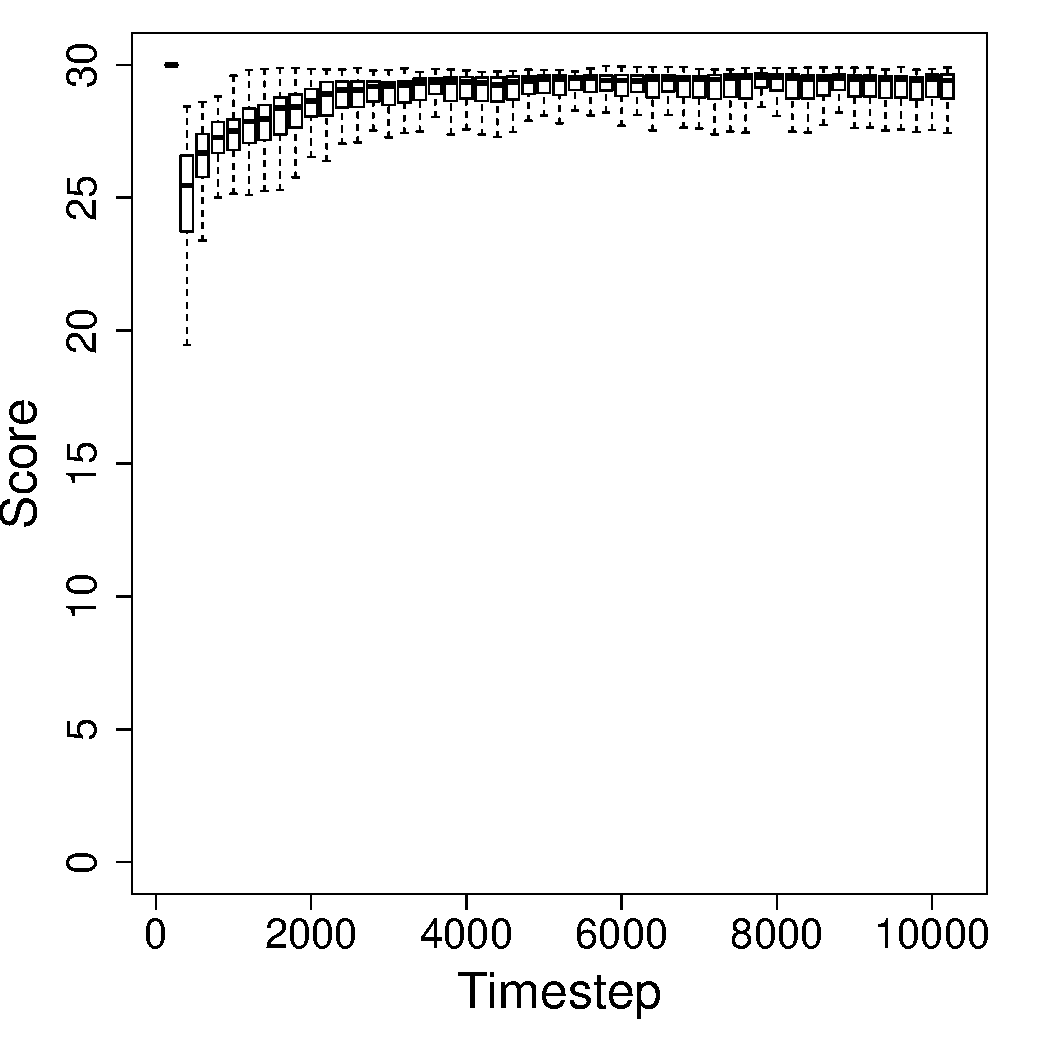
\includegraphics[width=.45\textwidth]{img/ScoreEvolutionForTrade-G3N500.pdf} \\
	\end{tabular}
	\vspace{-.5cm}
	\caption{
	    \small
	    Graphs from \cite{carrignon2015modelingthecoevolutionoftradeandcultureinpastsocieties}, left: evolution of prices toward clearing market prices. Right: evolution of agents score toward the optimal scores.
	}
	\label{fig:ratioEvol}
\end{figure}

In this original model, groups of agents produce, consume and exchange goods, and then adapt their trading strategies by \emph{innovating}, or by \emph{learning from someone else}. Those two later aspects are the cultural aspect we want to consider here. More specifically we restrain ourselves to the second one, the \emph{innovation process}. In all the simulations of this study the \emph{social learning mechanism} is the same: at some point, agents will copy the best agents in their social environment.

On the other side, the \emph{innovation process} is implemented as a probability $\mu$ that one agent randomly change the price he attributes to a good. This probability $\mu$ is what we call the innovation rate.

In the following sections we want to quantify the range of values for this parameter that allow the model to end in a GE.

\subsection*{Fitting to Idealized Outcomes}

To do so we apply a variation of \emph{Approximate Bayesian Computation} (ABC). ABC relies on Bayesian inference to compute and compare the likelihood of models to explain a set of empirical evidences under different parameter distributions. It has been already fruitfully applied to study changes in socio-cultural construct such as battlefield strategies~\cite{rubiocampillo2016modelselectioninhistoricalresearchusingapproximatebayesiancomputation}.

Here we use a slight variation of ABC, called \emph{Fitting to Idealized Outcomes} (FIO)~\cite{gallagher2015transitiontofarmingmorelikelyforsmallconservativegroupswithpropertyrightsbutincreasedproductivityisnotessential}, as it compares the parameter space of a model to the output of known theoretical model, instead of empirical evidence.

\vspace{.2cm}
{
	\footnotesize 
	FIO steps:
\vspace{-.3cm}
\setlength{\columnsep}{1mm}
	\begin{multicols*}{2}
	    \begin{enumerate}
		    \compresslist
		\item sample of $\mu$ with $\mu\sim U(0,1)$
		\item run simulations with innovation rate = $\mu$ 
		\item compute distance $\epsilon$ to idealize outcome~(GE):  
		    \begin{align*}
			\epsilon = \frac{ \sum_{i=1}^{n} s_i-s_{ge} }{n}   
		    \end{align*}
		    {\tiny ($n$: total number of agents, $s_i$ score of agent i, $s_{ge}$: ideal score)}
		    \vfill
		    \columnbreak
		\item select $200$ simulations with $\epsilon<.25$, 
		\item draw \emph{posterior} distribution of $\mu$ for those simulations.
	    \end{enumerate}
	\end{multicols*}
 }

 }




\headerbox{Results \& Analysis}{name=res1,column=1,span=1,row=.01}{

    The Figure~\ref{fig:abc} shows the results of the Fitting to Idealized Outcomes. The original model was run with 600 agents exchanging and producing 3 goods during $10\,000$ time steps. 
    
    The posterior distribution of the value of $\mu$ used by the best simulations clearly shows that only a restricted range of innovation rate allow the equilibrium to emerge. 
\begin{figure}[H]
	\centering
		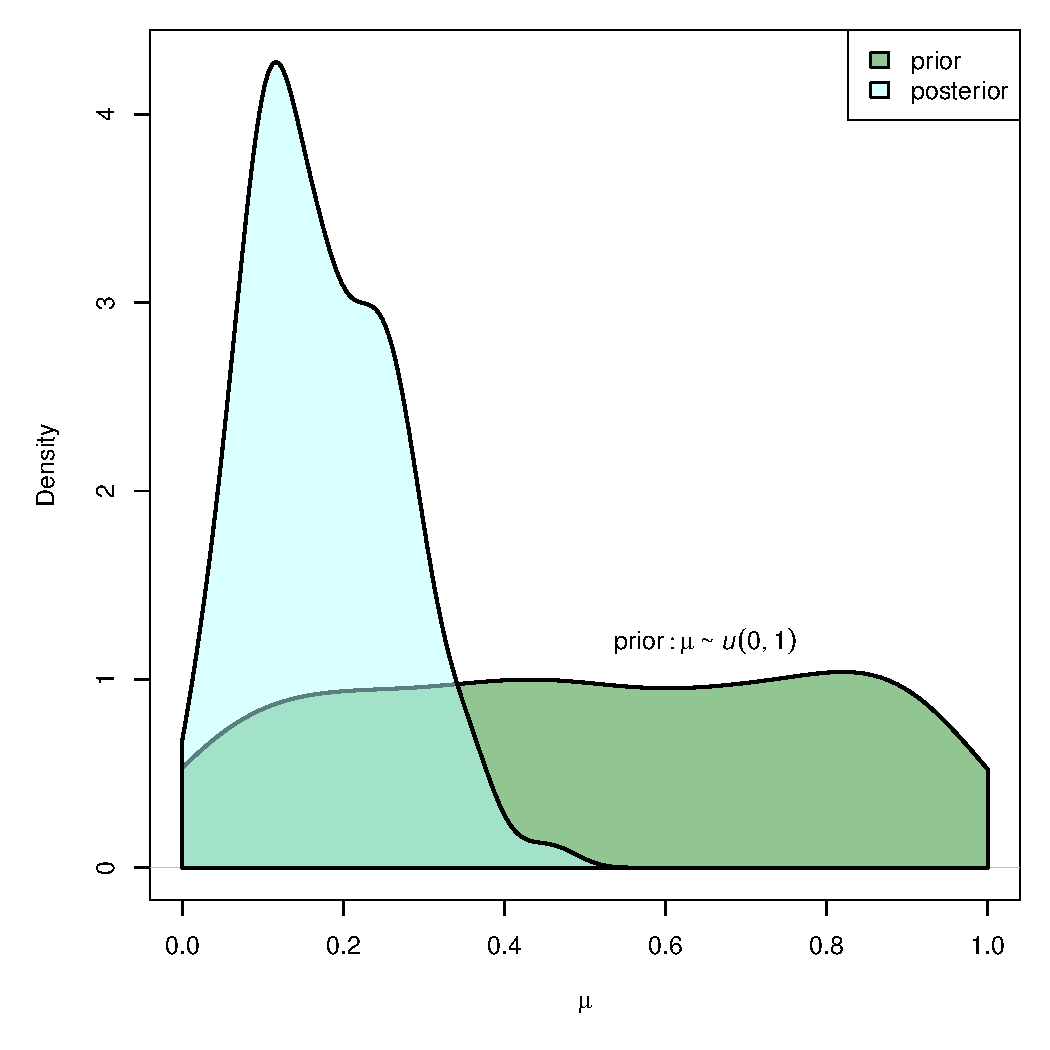
\includegraphics[width=.8\textwidth]{img/ABC.pdf} 
		\vspace{-.5cm}
		\caption{\small Result of the FIO: In green the prior distribution where $\mu$ is sampled from. In green the posterior distribution of $\mu$ for the $200$ simulations the closest to GE. }
		\label{fig:abc}
\end{figure}

    Without surprise this innovation rate has to be inferior to $0.5$, it would otherwise means that agents are changing their prices almost once every two time steps. This would make the result of any interaction between agents meaningless and would prevent any positive change to be fixed in the population.

On the other hand, this innovation rate remains pretty high: the mean value of $\mu$ for the best simulations is $0.175$, $ie$ a rate of change close to one change every 6 time steps. If this innovation rate has to be compared to the mutation process acting in biological evolution, our result are order of magnitude higher. This may underlie the difference of speed between biological and social process and the need for  social agents to quickly adapt to complex situations. 

At the same time, this high rate of random changes would be drastically reduced if our agents were able to made no-random innovation and use self-adapting strategy which are processes closer to what is observed in real systems.

}


\headerbox{Concluding Remarks}{name=conclusion,column=1,below=res1}{

This preliminary study shows how the use of simulation and model testing tools such as Fitting to Idealize Outcome, can help us articulate economic theory with other field. Coupled with empirical data and results from other experiments we could easily quantify if the right conditions were met in order to see the establishment of a General Equilibrium or not.

}


\headerbox{References}{name=references,column=1,below=conclusion}{
	\scriptsize
	\renewcommand{\refname}{\vspace{-0.5em}}
	\setlength{\parskip}{0pt}
	\setlength{\itemsep}{0pt}
	\bibliographystyle{abbrv}
	\bibliography{../../biblio/bib/SimonCarrignon,../../biblio/bib/phd,biblio}
}
\headerbox{Acknowledgements}{name=acknowledgements,column=1,below=references}{
    \small
    Funding for this work was provided by the ERC Advanced Grant EPNet (340828).
    \begin{center}
	\includegraphics[width=3cm]{epnetLogo.png}
	\includegraphics[width=2.5cm]{LOGO-ERC.jpg}
    \end{center}
} 

\end{poster}

\end{document}
